%%%%%%%%%%%%%%%%%%%% author.tex %%%%%%%%%%%%%%%%%%%%%%%%%%%%%%%%%%%
%
% sample root file for your "contribution" to a proceedings volume
%
% Use this file as a template for your own input.
%
%%%%%%%%%%%%%%%% Springer %%%%%%%%%%%%%%%%%%%%%%%%%%%%%%%%%%


\documentclass{svproc}
%\usepackage{marvosym}
%
% RECOMMENDED %%%%%%%%%%%%%%%%%%%%%%%%%%%%%%%%%%%%%%%%%%%%%%%%%%%
%
\usepackage{graphicx}
\usepackage{mathtools}
\usepackage{amsmath,amssymb,amsfonts}
\usepackage{algorithmic}
\usepackage{textcomp}
\usepackage{amsmath}
\usepackage{bbding}


% to typeset URLs, URIs, and DOIs
\usepackage{url}
\usepackage{hyperref}
\def\UrlFont{\rmfamily}
\providecommand{\doi}[1]{doi:\discretionary{}{}{}#1}

\def\orcidID#1{\unskip$^{[#1]}$}
\def\letter{$^{\textrm{(\Letter)}}$}

\begin{document}
\mainmatter              % start of a contribution
%
\title{Comparative Analysis of Parallel Computational Schemes for 
Solving the Time-consuming Decision Making Problems}
%
\titlerunning{Solving the Time-consuming Decision Making Problems}  % abbreviated title (for running head)
%                                     also used for the TOC unless
%                                     \toctitle is used
%
\author{Victor Gergel \orcidID{0000-0002-4013-2329} (\Envelope) \and
Evgeny Kozinov \orcidID{0000-0001-6776-0096}}
%
\authorrunning{Victor Gergel et al.} % abbreviated author list (for running head)
%
%%%% list of authors for the TOC (use if author list has to be modified)
\tocauthor{Victor Gergel and Evgeny Kozinov}
%
\institute{Lobachevsky State University of Nizhni Novgorod \\
Nizhni Novgorod, Russia \\
\email{gergel@unn.ru}, \email{evgeny.kozinov@itmm.unn.ru}}

\maketitle              % typeset the title of the contribution

\begin{abstract}
In the present paper, an efficient approach to the parallel solving of the complex multicriterial optimization problems using the heterogeneous computing systems is considered. The complexity of these problems can be very high as the optimized criteria can be multiextremal and the computing of the criteria values can be time-consuming.  In the framework of the proposed approach the multicriterial optimization problem is reduced to solving a series of global optimization problems by means of the convolution of the partial criteria with different sets of parameters. To solve the series of the global optimization problems, the efficient information-statistical global search method is applied.  The parallel computations are implemented by solving several global optimization problems simultaneously. The comparative analysis of various methods for parallel computations and numerous numerical experiments are presented in the paper.
\keywords{Decision making $\cdot$ Multicriteria global optimization $\cdot$ Parallel calculations $\cdot$ Dimensionality reduction $\cdot$ Search information $\cdot$ Numerical experiments}
\end{abstract}
%
\section{ Introduction}
\label{sec:01}
Decision making is inherent to almost all fields of human activities. A variety of the mathematical formulations have been proposed for the formal description of the decision making problems. Among these ones, there are many classes of optimization problems including unconstrained optimization, nonlinear programming, global optimization, etc. In the most complex situations of decision making, the multicriterial optimization (MCO) problem statements are used widely. An opportunity to set several criteria is a distinctive property of the MCO problems that allows more precise formulating the requirements to the optimality of chosen decisions. The MCO topic is a field of intensive studies - see, for example, the monographs \cite{x1,x2,x3,x4,x5,x6} and the reviews of the scientific and practical results in \cite{x7,x8,x9,x10}.

The possibility of contradictions between the partial criteria of efficiency that makes it impossible to achieve the optimal (the best) values for all partial criteria simultaneously is an important feature of the multicriterial optimization problems. As a result, the finding of some compromised (efficient, non-dominated) decisions, in which the achieved values with respect to some partial criteria satisfy given requirements to necessary level of efficiency, is taken as a solution of an MCO problem usually. 

The present work is devoted to solving the MCO problems, which are used for the description the decision making problems in the design of complex objects and systems. In such applications, the partial criteria can take a complex multiextremal form, and computing the values of the criteria and constraints may require a large amount of computations. 

Besides, within the framework of considered approach, an opportunity of correcting the MCO problem statements when changing the perceptions of the requirements to the optimality of the chosen decisions is allowed. Thus, in the case of redundancy of the partial criteria set, an opportunity to transform some criteria into the constraints is allowed. Or, otherwise, if the set of feasible variants is insufficient, some constraints can be transformed into the criteria, etc. Such an opportunity to change the MCO problem statements is an additional source of increased computational costs of the search for the optimal decisions. 

In the present paper, the results of the performed investigations on the generalization of the decision making problem statements \cite{x11,x12} and on the development of the highly efficient global optimization methods utilizing the whole search information obtained in the course of computations \cite{x13,x14,x15,x16,x17} are presented. 

Further structure of the paper is as follows. In Section \ref{sec:02}, the multicriterial optimization problem statement is given. In Section \ref{sec:03}, the reduction of the multicriterial problems to the scalar optimization ones by means of the minimax convolution of partial criteria and the dimensionality reduction with the use of Peano space-filling curves are considered. In Section \ref{sec:04}, the possibility of enhancing the efficiency of computations based on the reuse of the search information is substantiated. In Section \ref{sec:05}, the general organization scheme of parallel computations allowing the maximum use of the computational potential of modern supercomputer systems is described. Section \ref{sec:06} presents the results of numerical experiments supporting the proposed approach to be promising. In conclusion, the obtained results are discussed and possible main directions of further investigations are outlined.


\section{Multiple multicriterial optimization problem statement}
\label{sec:02}
For the formal description of the process of search for the efficient variants in complex decision making problems, the following generalized multilevel model is proposed.

1. At the highest level, within the framework of proposed model, a decision-making problem (DMP) is defined, for which a choice of the optimal values of the parameters should be done according to the available requirements to optimality. In the most general form, DMP can be defined with the use of a vector function of characteristics 
\begin{equation}
\label{eq:01}
w(y)=(w_1(y), w_2(y), \dots, w_M(y)), y \in D,
\end{equation}
where $y=(y_1,y_2, \dots ,y_N)$ is the vector of constructive parameters, and $D \in R^N$ is the domain of feasible values, which usually is a $N$-dimensional hyperinterval
\begin{equation}
\label{eq:02}
D=\{ y\in R^N : a_i \leq y_i \leq b_i,1 \leq i \leq N \},
\end{equation}
for given vectors $a$ and $b$. 

The values of characteristics $w(y)$ are supposed to be non-negative, and the decreasing of these ones corresponds to the increasing of the efficiency of the chosen variants. Also, it is supposed that the characteristics $w_j (y)$, $1 \leq j \leq M$ can be multiextremal and the computing of the values of these ones can require a large amount of computations. Besides, within the framework of considered approach, the characteristics $w_j(y)$, $1 \leq j \leq M$ are supposed to satisfy the Lipschitz condition 
\begin{equation}
\label{eq:03}
|w_j(y_1) - w_j(y_2)| \leq L_j \|y_1-y_2\|, 1 \leq j \leq M,
\end{equation}
where $L_j$ is the Lipschitz constant for the characteristic $w_j(y)$, $1 \leq j \leq M$, and  $\|*\|$ denotes the Euclidean norm in $R^N$. It is important to note that the fulfillment of the Lipschitz condition corresponds to the practical applications -- at small variations of the parameters $y \in D$ the corresponding variations of the values of characteristics $w_j(y)$, $1 \leq j \leq M$ are limited as a rule.
 
In general, the model of DMP is defined by the following set of elements 
\begin{equation}
\label{eq:04}
S=<y,w(y),D,a,b>.
\end{equation}

This model is supposed to remain the same and doesn\'t change in the course of computations.

2. The requirements to the optimality of the chosen variants $y \in D$ of the DMP can be defined in the following way. First of all, the characteristics $w_j(y)$, $1 \leq j \leq M$ should be selected, for which the achievement of the minimum possible values is necessary. Defining a set of indices $F=\{ i_1,i_2, \dots ,i_s \}$ of such characteristics defines the vector criterion of efficiency 
\begin{equation}
\label{eq:05}
f(y)=(w_{i_1}(y),w_{i_2}(y),\dots,w_{i_s}(y)).
\end{equation}

For the characteristics $w_j(y)$, $1 \leq j \leq M$ not included into the vector criterion of efficiency with the set of indices $G=\{ j_1,j_2, \dots ,j_m\}$ the sufficient levels of efficiency should be defined by a tolerance vector $q=(q_1,q_2,\dots,q_m)$. The availability of tolerances allows defining a vector function of constraints 
\begin{equation}
\label{eq:06}
g(y)= (g_1(y),g_2(y),\dots,g_m (y)), g_l (y) = w_{j_l}(y) - q_l, j_l \in G, 1 \leq l \leq m.
\end{equation}

The constraints $g(y)$ define the feasible search domain 
\begin{equation}
\label{eq:07}
Q=\{ y\in D:g(y) \leq 0 \}.
\end{equation}

The criteria of efficiency and constraints formulated in such a way allow formulating a multicriterial optimization (MCO) problem 
\begin{equation}
\label{eq:08}
f(y) \to min, y \in Q,
\end{equation}
defined on the basis of the model $S$ from (\ref{eq:04}) with the use of the elements listed above 
\begin{equation}
\label{eq:09}
P=<S,F,G,q>.
\end{equation}

The scheme proposed above covers many existing optimization problem statements. When $s=1$ and $m=0$ the general statement becomes the global optimization problem. When $s=1$ and $m>0$ the general statement defines a nonlinear programming problem. When $s>1$ and $m>0$ the general statement is reduced to a constrained multicriterial problem.

3.	The use of the multicriterial optimization problem statements reduces the complexity of the formal description of the decision making problems -- it becomes possible to define several partial criteria instead of necessity to define a unified ''global'' criterion of efficiency in the MCO problems. No doubt, such an approach is a simpler task for the decision maker determining the requirements to the optimality of the decisions made. It is worth noting also that the multicriterial definition of the efficiency criteria corresponds to the practice of decision making in various fields of applications.

The scheme of the MCO problem statement considered above has been proposed first in \cite{x11} and was used widely in solving many applied decision making problems. At the same time, the results of the practical application of the approach have demonstrated that the formulating of a single MCO problem statement might also appear to be difficult when altering the ideas of the necessary requirements to the optimality. Thus, in the case of redundancy of the partial criteria set, the transformation of some criteria into the constraints may appear to be appropriate. Or, vise versa, if a small feasible domain $Q$ is obtained, the loosening of the tolerances $q$ or transforming some constraints into the criteria may be required. As a result, an opportunity of simultaneous formulating several MCO problems 
\begin{equation}
\label{eq:10}
\mathbb{P}_t=\{P_1,P_2,\dots,P_t\}
\end{equation}
will be allowed  within the framework of the extended model of the optimal choice as further development of the scheme (\ref{eq:01})-(\ref{eq:09}). It is worth noting that the set of problems $\mathbb{P}$ can change in the course of computations by means of adding new problems 
\begin{equation}
\label{eq:11}
\mathbb{P}'=\mathbb{P}+/-\mathbb{P}.
\end{equation}
or removing already existing ones. Solving the problems from the set $\mathbb{P}$ can be performed sequentially or simultaneously in the time-sharing mode or in parallel if several computing devices are available. No doubt, the simultaneous method of solving the problems is more preferable -- the results obtained in the course of computations allow adjusting current set of problems $\mathbb{P}$ promptly. In the case of utilizing the parallel computations, the total time of problem solving can be reduced essentially.

In general, the proposed model of the process of search for the optimal decisions (\ref{eq:01})-(\ref{eq:11}) defines a new class of the optimization problems -- the multiple multicriterial global optimization (MMGO) problems.

\section{Successive reduction of the multicriterial global optimization problems }
\label{sec:03}

As it has been already mentioned above, the partial criteria of efficiency in the MCO problems are contradictory usually. This feature of the MCO problems means that the obtaining of the optimal (the best) values with respect to all partial criteria simultaneously cannot be ensured. In such situation, the finding of particular compromised (effective, non-dominated) decisions, in which the achieved values with respect to particular partial criteria cannot be improved without simultaneous worsening with respect to some other criteria is understood as the solution of a MCO problem usually. In the limiting case, the finding of all effective (Pareto-optimal) decisions $PD(Q) \subset Q$. can be required.

Due to a high relevance, a large enough quantity of methods of solving the MCO problems have been developed and used widely -- see, for example, \cite{x2,x3,x4,x5,x6,x7,x8,x9,x10}. A part of these algorithms ensures the obtaining the numerical estimates of the whole Pareto set $PD(Q)$ \cite{x3,x26,x27,x28}. Along with the usefulness of such an approach (all effective decisions of the MCO problem are found), the use of these methods appears to be difficult often because of high computational complexity of obtaining the estimates of the Pareto set. Besides, the estimate of the whole set $PD(Q)$ may appear tо be redundant when to solve the MCO problem it is enough to obtain several particular effective decisions (that takes place in the practical applications often). As a result, more widely used approach to solving the MCO problems is based on the scalarization of the vector criterion into some general scalar criterion of efficiency, the optimization of which can be performed with the use of already existing optimization methods. Among these methods, for example, there are weighted sum method, compromise programming method, weighted min-max method, goal programming, and many other algorithms -- see, for example, \cite{x2,x3,x4,x5,x6}. 

The general approach used in the present work consists in the reduction of solving a MMGO problem to the solving of a series of single-criterion global optimization problems \footnote{Due to initial assumptions on possible multiextremality of the characteristics $w_j(y), 1 \leq j \leq M$ from (\ref{eq:01})}: 
\begin{equation}
\label{eq:12}
\min {\varphi(y)}=F(\lambda,y), g(y) \leq 0, y \in D, 
\end{equation}
where $g(y)$ is the vector function of constraints from (\ref{eq:06}), and $F(\lambda,y)$ is the minimized convolution of the partial criteria $f_i(y(x))$, $1 \leq i \leq s$ of the MCO problem (\ref{eq:05})
\begin{equation}
\label{eq:13}
F(\lambda,y)=\max{⁡(\lambda_i f_i (y), 1 \leq i \leq s)} 
\end{equation}
using the vector of the weighting coefficients 
\begin{equation}
\label{eq:14}
\lambda=(\lambda_1, \lambda_2, \dots , \lambda_s )\in \Lambda \subset R^s: \sum_{i=1}^s{\lambda_i=1}, \lambda_i \geq 0, 1 \leq i \leq s.
\end{equation}

In the developed approach, it is proposed to perform one more step of conversion of the problems $F(\lambda,y)$ from (\ref{eq:12}) being solved -- to perform the dimensionality reduction using the Peano space-filling curves (evolvents) $y(x)$ providing an unambiguous mapping of the interval $[0,1]$ onto an $N$-dimensional hypercube D \cite{x18,x20}. As a result of such reduction, the multidimensional global optimization problem (\ref{eq:12}) is reduced to the one-dimensional problem:
\begin{equation}
\label{eq:15}
F(\lambda,y(x^*)) = \min{\{F(\lambda,y(x)): g(y(x)) \leq 0, x \in [0,1]\}}.
\end{equation}

The considered dimensionality reduction scheme superimposes the multidimensional problem with the Lipschitzian minimized function $F(\lambda,y)$ to a one-dimensional problem, in which the reduced function $F(\lambda,y(x))$ satisfies the uniform H\"{o}lder condition i.e.
\begin{equation}
\label{eq:16}
|F(\lambda,y'(x)) - F(\lambda, y''(x))| \leq H \|x' - x''\|, x', x'' \in [0,1], 
\end{equation}
where the constant $H$ is defined by the relation $H=2L\sqrt{N+3}$, $N$ is the dimensionality of the optimization problem from (\ref{eq:01}), and $L$ is the Lipschitz constant of the function $F(\lambda,y)$ from (\ref{eq:12}). The dimensionality reduction allows applying many well known highly efficient one-dimensional global optimization algorithms for solving the problems (\ref{eq:12}) (after performing the necessary generalization) -- see, for example, \cite{x18,x20,x29,x30,x31,x32,x33,x34,x35}.

In order to obtain several effective decisions (or to estimate the whole Pareto domain) the problem (\ref{eq:12}) should be solved several times for corresponding sets of the values of the elements of the weighting vector $\lambda \in \Lambda$. In this case, the set of MCO problems $\mathbb{P}$ from (\ref{eq:10}) necessary for solving the initial decision making problem is transformed into a wider set of scalar optimization problems (\ref{eq:12})
\begin{equation}
\label{eq:17}
\mathbb{F}_T=\{F_i (\lambda_i,y): \lambda_i \in \Lambda, 1 \leq i \leq T \},
\end{equation}
where several problems (\ref{eq:12}) with different values of the coefficients $\lambda \in \Lambda$ can correspond to each problem $P \in \mathbb{P}$.

\section{Improvement the efficiency of computations based on the reuse 
of the search information} 
\label{sec:04}
As it has been already mentioned above, the solving of the MCO problems $P$ from (\ref{eq:10}) and corresponding global optimization problems $F$ from (\ref{eq:15}) can require a large amount of computations even when solving a single particular problem. In the case if a series of problems from the sets $\mathbb{P}$ and $\mathbb{F}$ should be solved, the necessary amount of computations could appear to be even larger. And, therefore, overcoming the computational complexity of the decision making problems of the considered class is a necessary condition of opportunity of a practical application of the proposed approach. An intensive use of the whole search information obtained in the course of computations can be a promising approach to solving this problem. 

The numerical solving of the global optimization problems is reduced usually to a sequential computing the values of characteristics $w(y)$ at the points $y^i$, $0\leq i \leq k$ of the search domain $D$ \cite{x18,x22,x23,x24,x25}. The data obtained as a result of computations can be represented in a form of matrix of search information (MSI)
\begin{equation}
\label{eq:18}
\Omega_k=\{(y^i,w^i=w(y^i ) )^T:1 \leq i \leq k\}.
\end{equation}

As a result of scalarization of the vector criterion (\ref{eq:12}) and application of the dimensionality reduction (\ref{eq:15}), $\Omega_k$ from (\ref{eq:18}) can be transformed into the form of the matrix of the search state (MSS):
\begin{equation}
\label{eq:19}
A_k=\{(x_i,z_i,g_i,l_i )^T:1 \leq i \leq k\},
\end{equation}
where
\begin{itemize}
	\item $x_i$, $1 \leq i \leq k$ are the reduced points of the executed global search iterations where the criteria values have been computed; 
	\item $z_i$, $g_i$, $1 \leq i \leq k$ are the values of the scalar criterion and of the constraints at the points $x_i$, $1 \leq i \leq k$ for current optimization problem $F(\lambda,y(x))$ from (\ref{eq:15}) being solved i. e.
\begin{equation}
z_i = \varphi(x_i) =F(\lambda,y(x_i)),  g_i=g(y(x_i )),  1\leq i \leq k;
\end{equation}
	\item $l_i$, $1 \leq i \leq k$ are the indices of the global search iterations, at which the points $x_i$, $1 \leq i \leq k$ have been generated, these indices are used to storing the correspondence between the reduced points and the multidimensional ones at the executed iterations i. e.
\begin{equation}
y^j = y(x_i), j = l_i, 1 \leq i \leq k.
\end{equation}

\end{itemize}

The matrix of the search state $A_k$ contains the search information transformed to current scalar reduced problem (\ref{eq:15}) being solved. Besides, the search information in the MSS is arranged according to the values of coordinates of the points $x_i$, $1 \leq i \leq k$ for more efficient execution of the global search algorithms; the arranged representation of the points is reflected by the use of the lower index i. e.
\begin{equation}
x_1 \leq x_2 \leq \dots \leq x_k.
\end{equation}

The representation of the search information obtained in the course of computations in the form of  the matrices $\Omega_k$ and $A_k$ makes the basis for the development of efficient optimization search procedures. The availability of such information allows performing an adaptive choice of the points for executing the global search iterations taking into account the results of all computations completed earlier 
\begin{equation}
\label{eq:20}
y^{k+1}=Y(\Omega_k),k=1,2,\dots.
\end{equation}
where $Y$ is the rule for computing the points $y^i$, $0 \leq i \leq k$ of the applied optimization algorithm. Such an adaptive choice of the points of executed search iterations can accelerate the finding of the effective decisions. In the case of the global optimization problems, the accumulation of the whole search information and the use of the rules of the kind (\ref{eq:20}) is just mandatory. Any reduction of the search information in determining the points to be executed would result in executing the excess global search iterations.

It should be noted that the availability of MSS $\Omega_k$ from (\ref{eq:18}) allows reducing the results of all preceding computations $z_i$,  $1 \leq i \leq k$ stored in the MSS $A_k$ to the values of current optimization problem $F(\lambda,y(x))$ from (\ref{eq:15}) being solved for any new parameter of the MCO problem statement $P$ from (\ref{eq:09}) and for any new value of the convolution coefficients $\lambda$ from (\ref{eq:14}) on the basis of the values of characteristics $w^i$, $1 \leq i \leq k$ computed earlier and stored in $\Omega_k$ without any repeated time-consuming computation of the values of $w(y)$ from (\ref{eq:01}) i.e.
\begin{equation}
\label{eq:21}
w_i \xrightarrow{\lambda,P} (z_i,g_i ), 1 \leq i \leq k,\forall \lambda \in \Lambda, P \in \mathbb{P}.
\end{equation}

Therefore, all the search information can be employed for continuing the computations in full amount. An efficient use of this information becomes an important requirement in the selection of the methods for solving the problems $F(\lambda,y(x))$ from (\ref{eq:15}). The reuse of the search information can provide a continuous decreasing of the amount of computations for solving every next optimization problem up to execution of just few iterations only to find the next effective decision.

\section{Parallel computations in the multiple multicriterial global optimization problems} 
\label{sec:05}

The sequential solving the set of problems $\mathbb{F}$ from (\ref{eq:17}) to find several globally optimal decisions increases the amount of computations required to solve the decision making problems essentially. The parallel solving of the problems $F(\lambda,y(x))$ from the set $\mathbb{F}$ is a promising and simple method of accelerating the performed computations. At high enough number of the computer nodes (processors), the time of solving the whole set of problems $\mathbb{F}$ would be determined by the computation time for the problem $F(\lambda,y(x))$, the solving of which takes the longest time. Such an approach can be implemented quite easily. However, it doesn\'t solve the problem of computational complexity when it is necessary to expand the set of problems $\mathbb{F}$ in the course of computations.

The method of organizing the parallel computations considered above can be developed further by utilizing the information compatibility of the problems from the set $\mathbb{F}$ -- as has been noted in Section {\ref{sec:04}}, the values of characteristics $w^i$, $1 \leq i \leq k$ computed when solving any problem $F_1(\lambda,y(x))$ can be transformed to the values of any other problem $F_2(\lambda,y(x))$. This result allows proposing the following general scheme of parallel computations for simultaneous solving the problems from the set $\mathbb{F}$.

\textbf{1. The distribution of problems.} Prior to the start of computations, the problems of the set $\mathbb{F}$ from (\ref{eq:17}) should be distributed among the computational nodes of a multiprocessor system. This distribution can be quite diverse -- for solving a particular problem from the set $\mathbb{F}$, various numbers of computational cores $(q, q \geq 1)$ and of the computational nodes $(p, p \geq 1)$ can be allocated. An opportunity to use several computational nodes $p>1$ for solving the same problem is provided by means of application of multiple evolvents $y_i (x)$, $1\leq i\leq p$ -- see \cite{x13,x14}. If when solving a particular problem from the set $\mathbb{F}$ it is planned not to employ the processor cores of a computational node in full, in this case several optimization problems can be being solved using the same node subject to the number of processors available on the computational node and to the number of computational cores in each processor. 

\textbf{2. The choice of the optimization algorithms.} The proposed scheme of the parallel computations is a general one -- various methods of multiextremal optimization can be applied for solving the problems on each computational node -- see, for example, \cite{x18,x20,x29,x30,x31,x32,x33,x34,x35}. The main requirement to the selection of the algorithms -- the methods should use the search information $\Omega
_k$ and $A_k$ to increase the efficiency of global search. And, as it has been already noted above in Section \ref{sec:03}, the global optimization algorithms should be generalized in order to provide solving the reduced one-dimensional global optimization problems of the kind $F(\lambda,y(x))$ from the set $\mathbb{F}$. The possibility of application of the proposed approach was substantiated using the example of the efficient global search algorithms developed within the framework of the information-statistical theory of the multiextremal optimization -- see \cite{x12,x13,x14,x15,x16,x17,x18}.

\textbf{3. The execution of the global search iterations.} The execution of the global search iterations for each problem $F(\lambda,y(x))$ from the set $\mathbb{F}$ being solved is performed in parallel. The execution of every iteration on each computational node includes performing the following operations:
\begin{enumerate}
	\item The choice of $q$, $q \geq 1$ points $x^i$, $1\leq i\leq q$ of the next global search iteration is performed according to the rule (\ref{eq:20}) of the optimization method; the choice of the points is performed taking into account the available search information $\Omega_k$ and $A_k$; the number of generated points $q$, $q\geq 1$ is determined by the number of computational cores employed for solving the problem $F(\lambda,y(x))$;
	\item For each chosen one-dimensional point $x^i \in [0,1]$, $1 \leq i \leq q$ of current global search iteration, the multidimensional image $y^i \in D$, $1 \leq i \leq q$ is determined according to the mapping $y(x)$. Then, each computed image $y^i \in D$, $1 \leq i \leq q$ is transmitted to all employed computational nodes to avoid the multiple choice of the same points in the domain $D$ when solving the problems from the set $\mathbb{F}$;
	\item The values of characteristics $w(y)$ from (\ref{eq:01}) are computed at all points $y^i \in D$, $1 \leq i \leq q$; for each particular point $y^i \in D$, $1 \leq i \leq q$, these computations are performed in parallel using different computational cores; the computed values of characteristics $w(y)$ are transmitted to all employed computational nodes to include the obtained data into the search information $\Omega_k$ and $A_k$.
\end{enumerate}

\textbf{4. Updating the search information.} Prior to starting the next global search iteration, the availability of data transmitted from other computational units (processors or cores) is checked; the received data should be included into the search information.

According to the presented computational scheme of parallel computations, each computational unit would contain the identical copies of the matrix of search information $\Omega_k$ from (\ref{eq:18}); the matrices $A_k$ from (\ref{eq:19}) would contain different sets of the global search points $x_i$, $1\leq i\leq k$ because of the use of different evolvents $y(x)$ for the dimensionality reduction and of different values of the scalar criterion and constraints $z_i$, $g_i$, $1\leq i\leq k$ corresponding to the problems $F(\lambda,y(x))$ from the set $\mathbb{F}$ being solved.

Within the framework of such computational scheme, it becomes possible to expand the set of problems being solved $\mathbb{F}$ at any moment of computations -- in order to solve a new problem $F(\lambda,y(x))$, it is enough to allocate an additional computational unit, to copy the set $\Omega_k$, and to create the corresponding matrix $A_k$.

It is clear that the increase of the efficiency of the global search due to the use of the sets of the search information $\Omega_k$ and $A_k$ depends on the optimization algorithms employed. The analysis of the elements of the scheme of organization of the parallel computations considered above in application to the information-statistical global optimization algorithms has been performed in \cite{x12,x13,x14,x15,x16,x17}. The results of numerical experiments carried out for complete experimental evaluation of the efficiency of the proposed scheme to choose the best parameters of the use of the computational resources of the high-performance supercomputer systems are presented below in Section \ref{sec:06}.



\section{The results of numerical experiments }
\label{sec:06}

The numerical experiments have been carried out using ''Lobachevsky'' supercomputer at University of Nizhni Novgorod (operation system -- CentOS 6.4, management system -- SLURM). Each supercomputer node had 2 Intel Sandy Bridge E5-2660 processors (2.2 GHz, 64 Gb RAM). Each processor included 8 cores (i.e. total 16 CPU cores were available at each computer node). In order to generate the executable program code, Intel C++ 17.0 compiler was used.

When performing the numerical experiments, according to the general scheme of parallel computations considered in Section \ref{sec:05}, the efficient algorithms of multicriterial multiextremal optimization \cite{x12,x13,x14,x15,x16,x17} developed within the framework of the information-statistical theory of global optimization \cite{x18} were used. The efficiency of these algorithms has been proven by many numerical experiments.

In the present work, the results of a series of the numerical experiments performed in order to choose the best parameters of the parallel computations (the number of employed computational cores and computer nodes, the number of the multicriterial optimization subproblems solved simultaneously, the number of evolvents used for the dimensionality reduction, etc.) are presented. Each experiment included the solving of 30 MCO problems. Each problem was a six-dimensional and five-criterial one i.e. $N=6$, $s=5$. The multiextremal functions defined by the GKLS generator \cite{x36} were used as the criteria. This generator allows generating the multiextremal optimization problems with the properties known a priori: the number of local minima, the sizes of their attractors, the global minimum point, the objective function value at this point, etc. 
%Some example contour plots of the functions obtained by the GKLS generator are presented in Fig. \ref{fig:01}. 
%\begin{figure}[htbp]
%\centerline{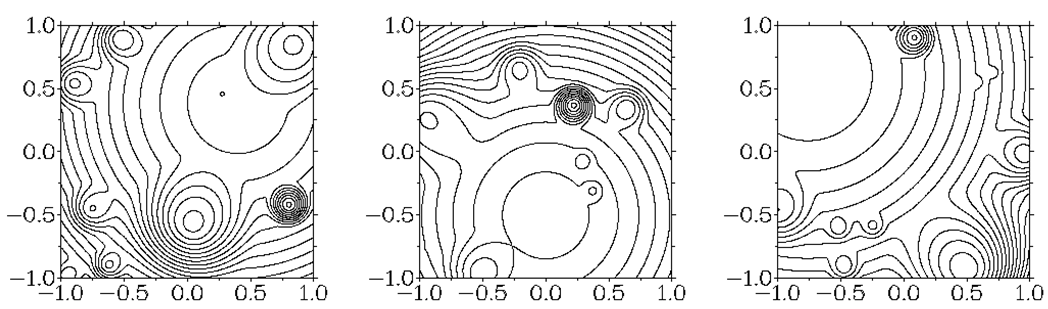
\includegraphics[width=0.7\textwidth]{fig1.png}}
%\caption{Contour plots of three multiextremal functions from the GKLS family of test optimization problems}
%\label{fig:01}
%\end{figure}

The following values of parameters were used in the numerical experiments. When solving the MCO problems, the condition of stopping the computations according to predefined accuracy $\varepsilon=0.05$ was used. For constructing the estimates of the Pareto domain $PDA(f,D)$, 100 subproblems of the family $\mathbb{F}$ from (\ref{eq:17}) have been solved for various values of the coefficients $\lambda \in \Lambda$. In the performed experiments, 10 computational nodes of the supercomputer were used, each computational node included two 8-core processors (i.e. total 160 computational cores were employed for performing the computations in each experiment). 

In the beginning of the performed series of experiments, the parallel computations have been conducted using a single supercomputer node only (two processors, 16 computational cores using the shared memory). The results of these experiments are presented in Table \ref{tab:02}.

%Table 2. Evaluation of the efficiency of using a single supercomputer node when solving 
%a series of 30 six-dimensional five-criterial MCO problems
%Cores	Search information	Iterations	S1	S2
%1	not used	26 813 722.7	1.0	
%1	used 	9 103 069.6	2.9	1.0
%8	used 	1 291 720.0	20.8	7.0
%16	used 	609 169.5	44.0	14.9
\begin{table}[htbp]
\centering
\caption{Evaluation of the efficiency of using a single supercomputer node when solving a series of 30 six-dimensional five-criterial MCO problems}
\label{tab:02}
\begin{tabular}{ccccc}
\hline
Cores & Search information & Iterations   & S1   & S2   \\ \hline
1     & not used           & 26 813 722.7 & 1.0  &      \\
1     & used               & 9 103 069.6  & 2.9  & 1.0  \\
8     & used               & 1 291 720.0  & 20.8 & 7.0  \\
16    & used               & 609 169.5    & 44.0 & 14.9 \\ \hline
\end{tabular}
\end{table}

In Table \ref{tab:02}, the number of computational cores employed when carrying out the experiments is presented in the \textit{Cores} column. The \textit{Search information} column contains the information on the reuse of the search information when solving the series of subproblems of the family $\mathbb{F}$ from (\ref{eq:17}) for different values of the coefficients $\lambda \in \Lambda$. The \textit{Iterations} column presents the average number of the global search iterations executed when solving particular subproblems of the MCO problem. The \textit{S1} column shows the overall speedup achieved by means of performing the parallel computations using the corresponding quantity of the computational cores. The \textit{S2} column contains the speedup of computations with respect to the serial optimization algorithm, in which the search information is used. 

As follows from the results presented in Table \ref{tab:02}, when using even a single computational core, one can achieve a speedup of computations almost by a factor of three by means of the reuse of the search information obtained in the course of optimization. The overall speedup achieved in the parallel computations makes 44 times using 16 cores of a single supercomputing node.

Further, in all experiments 10 supercomputer nodes were used (i. e. total 160 computational cores were employed). The parameters of the experiments were: the number of subproblems of the family $\mathbb{F}$ from (\ref{eq:17}) being solved simultaneously, the number of computational nodes employed for solving particular MCO subproblems, and the number of test problems (generated by the GKLS generator) being solved simultaneously (total 30 six-dimensional five-criterial test MCO problems were solved in each experiment). The results of the numerical experiments are presented in Table \ref{tab:03}.
%
%Table 3. Evaluation of efficiency of using ten supercomputing nodes when solving a series 
%of 30 six-dimensional five-criterial MCO problems
%Nodes	NumMCO	SubProblems	SubNodes	Iterations	S1	Scaling
%1	1	1	1	609 169.5	44.0	1.0
%10	1	10	1	75 045.8	357.3	8.1
%10	1	5	2	77 643.6	345.3	7.8
%10	1	1	10	108 700.0	246.7	5.6
%10	2	5	1	76 819.0	349.1	7.9
%10	2	1	5	81 132.8	330.5	7.5
%10	5	2	1	66 618.6	402.5	9.1
%10	5	1	2	77 995.0	343.8	7.8
%10	10	1	1	73 999.7	362.3	8.2
\begin{table}[htbp]
\centering
\caption{Evaluation of efficiency of using ten supercomputing nodes when solving a series of 30 six-dimensional five-criterial MCO problems}
\label{tab:03}
\begin{tabular}{ccccccc}
\hline
Nodes       & NumMCO     & SubProblems & SubNodes   & Iterations        & S1             & Scaling      \\ \hline
1           & 1          & 1           & 1          & 609 169.5         & 44.0           & 1.0          \\
10          & 1          & 10          & 1          & 75 045.8          & 357.3          & 8.1          \\
10          & 1          & 5           & 2          & 77 643.6          & 345.3          & 7.8          \\
10          & 1          & 1           & 10         & 108 700.0         & 246.7          & 5.6          \\
10          & 2          & 5           & 1          & 76 819.0          & 349.1          & 7.9          \\
10          & 2          & 1           & 5          & 81 132.8          & 330.5          & 7.5          \\
\textbf{10} & \textbf{5} & \textbf{2}  & \textbf{1} & \textbf{66 618.6} & \textbf{402.5} & \textbf{9.1} \\
10          & 5          & 1           & 2          & 77 995.0          & 343.8          & 7.8          \\
10          & 10         & 1           & 1          & 73 999.7          & 362.3          & 8.2          \\ \hline
\end{tabular}
\end{table}

The number of employed supercomputing nodes is given in the \textit{Nodes} column. In the \textit{NumMCO} column, the number of test MCO problems (generated by the GKLS generator) solved simultaneously is given. In the \textit{SubProblems} column, the number of subproblems of the family $\mathbb{F}$ from (\ref{eq:17}) solved simultaneously is presented. In the \textit{SubNodes} column, the number of the computational nodes employed for the solving of particular MCO subproblems is presented. The \textit{Iterations} column presents the averaged number of the global search iterations executed when solving particular subproblems of the MCO problem. The \textit{S1} column shows the overall speedup achieved by means of performing the parallel computations with the use of the corresponding quaintly of the supercomputing nodes. The \textit{Scaling} column contains the speedup of the parallel computations with respect to the results obtained when using a single computational node only.

As follows from the results presented in Table \ref{tab:03}, the best speed up in the considered series of experiments has been achieved at the simultaneous solving of five MCO problems of the test class when two subproblems of the family $\mathbb{F}$ from (\ref{eq:17}) are solved in parallel for each problem using a single supercomputing node for each subproblem (the parameters for this experiments are highlighted by the bold color in Table \ref{tab:03}). In this case, the speedup achieved for the parallel computations exceeds 400 (it should be noted that total 10 computational nodes including total 160 cores were used in this experiment).



\section{Conclusion }
\label{sec:07}


In the present paper, an efficient computational scheme of the parallel computations for solving the complex multicriterial optimization problems with the non-convex constraints, in which the optimization criteria can be multiextremal and computing the criteria values can require a large amount of computations is proposed. The proposed approach is based on the reduction of the multicriterial problems to the nonlinear programming ones by the minimax convolution of the partial criteria, the dimensionality reduction using the Peano space-filling curves, and application of the efficient information-statistical global optimization methods using a novel index scheme of accounting for the constraints instead of the penalty functions used commonly.

The developed general computational scheme includes the concurrent parallel computational methods for the computational systems with the shared memory, the distributed parallel computations using the multiple mappings for the dimensionality reduction, and the multilevel nesting of the parallel computations for the high-performance computational systems. In general, the proposed computational scheme ensures the opportunity of an efficient application of the high-performance computational systems with a large number (tens and hundreds thousand) cores/processors for solving the complex global optimization problems. Besides, this general scheme can be used for the organization of the parallel computations for a wide range of algorithms for solving the time-consuming problems of decision making (in particular, for the information-statistical global optimization algorithms). 

In order to determine the optimal parameters of the parallel computations, a series of experiments has been carried out. The results have shown the developed approach to allow reducing the computational costs of solving the multicriterial optimization problems with non-convex constraints considerably.

In conclusion, one can note the developed approach to be promising and requires further investigations. First of all, it is necessary to continue carrying out the numerical experiments on solving the multicriterial optimization problems for a larger quantity of partial criteria of efficiency and for larger dimensionality of the optimization problems being solved. 

\section*{Acknowledgements}  
This research was supported by the Russian Science Foundation, project No 16-11-10150 ''Novel efficient methods and software tools for time-consuming decision making problems using supercomputers of superior performance.''





%
% ---- Bibliography ----
%
\bibliographystyle{spmpsci}
\begin{thebibliography}{6}
%

%\bibitem {czaj:fitz}
%Czajkowski, K., Fitzgerald, S., Foster, I., Kesselman, C.: Grid information services
%for distributed resource sharing. In: Proceedings 10th IEEE International Symposium
%on High Performance Distributed Computing, pp. 181--184. IEEE, New York (2001).
%\doi{10.1109/HPDC.2001.945188}
%
%\bibitem {fost:kes}
%Foster, I., Kesselman, C. (eds.): The grid: blueprint for a new computing infrastructure.
%Morgan Kaufmann, San Francisco, CA, USA (1999)
%
%\bibitem {fo:kes:nic:tue}
%Foster, I., Kesselman, C., Nick, J., Tuecke, S.: The physiology of the grid: an open grid services architecture for distributed systems integration. Tech. rep., Global Grid
%Forum (2002)
%
%\bibitem {may:ehr:stein}
%May, P., Ehrlich, H.-C., Steinke, T.: ZIB structure prediction pipeline:
%composing a complex biological workflow through web services.
%In: Nagel, W.E., Walter, W.V., Lehner, W. (eds.) Euro-Par 2006.
%LNCS, vol. 4128, pp. 1148--1158. Springer, Heidelberg (2006).
%\doi{10.1007/11823285\_121}
%
%\bibitem {onlyurl}
%NCBI: National Center for Biotechnology Information. \url{http://www.ncbi.nlm.nih.gov}
%
%\bibitem {smit:wat}
%Smith, T.F., Waterman, M.S.: Identification of common molecular subsequences.
%Journal of Molecular Biology. \textbf{147}(1), 195--197 (1981). \doi{10.1016/0022-2836(81)90087-5}


\bibitem {x1} Parnell, G.S., Driscoll, P.J., Henderson, D.L., editors.: Decision Making in Systems Engineering and Management. Wiley, New Jersey (2nd ed., 2011).
\bibitem {x2} Miettinen K.: Nonlinear Multiobjective Optimization. Springer (1999).
\bibitem {x3} Marler, R. T., Arora, J. S.: Multi-Objective Optimization: Concepts and Methods for Engineering. VDM Verlag (2009).
\bibitem {x4} Ehrgott, M.: Multicriteria Optimization. Springer (2nd ed., 2010).
\bibitem {x5} Collette, Y., Siarry, P.: Multiobjective Optimization: Principles and Case Studies (Decision Engineering). Springer (2011).
\bibitem {x6} Pardalos, P.M., {\v Z}ilinskas, A., {\v Z}ilinskas, J.: Non-Convex Multi-Objective Optimization. Springer (2017). 
\bibitem {x7} Figueira,J., Greco, S., Ehrgott, M., editors.: Multiple criteria decision analysis: State of the art surveys. New York, Springer (2005).
\bibitem {x8} Hillermeier, C., Jahn, J.: Multiobjective optimization: survey of methods and industrial applications. Surv. Math. Ind. \textbf{11}, 1--42 (2005).
\bibitem {x9} Zavadskas, E. K., Turskis, Z., Kildiene, S.: State of art surveys of overviews on MCDM/MADM methods. Technological and Economic Development of Economy \textbf{20}, 165--179 (2014).
\bibitem {x10}Cho, J.-H., Wang, Ya., Chen, I.-R., Chan, K.S., Swami, A.: A Survey on Modeling and Optimizing Multi-Objective Systems. IEEE Communications Surveys \& Tutorials \textbf{19}(3), 1867--1901 (2017). 
\bibitem {x11}Strongin, R.G., Gergel, V.P. Markin, D.L.:  Multicriterion multiextreme optimization with nonlinear constraints. Lecture Notes in Economics and Mathematical Systems, \textbf{351}, 120--127 (1988).
\bibitem {x12}Gergel, V.P., Kozinov, E.A.: Accelerating multicriterial optimization by the intensive exploitation of accumulated search data. AIP Conference Proceedings \textbf{1776}, 090003 (2016). \doi{10.1063/1.4965367}
\bibitem {x13}Gergel, V.P., Kozinov, E.A.: Efficient multicriterial optimization based on intensive reuse of search information. J. Glob. Optim. \textbf{71}(1), 73--90 (2018). \doi{doi.org/10.1007/s10898-018-0624-3}
\bibitem {x14}Gergel, V.P., Kozinov, E.A.: Accelerating Parallel Multicriterial Optimization Methods Based on Intensive Using of Search Information. Procedia Computer Science, \textbf{108}, 1463--1472 (2017).
\bibitem {x15}Gergel, V., Kozinov, E.: Parallel computing for time-consuming multicriterial optimization problems. LNCS, \textbf{10421}, 446--458 (2017).  \doi{10.1007/978-3-319-62932-2\_43}
\bibitem {x16}Gergel, V., Kozinov, E.: Efficient methods of multicriterial optimization based on the intensive use of search information. Springer Proceedings in Mathematics and Statistics, \textbf{197}, 27--45 (2017). \doi{10.1007/978-3-319-56829-4\_3}
\bibitem {x17}Gergel, V., Kozinov, E.: An approach for parallel solving the multicriterial optimization problems with non-convex constraints. Communications in Computer and Information Science, \textbf{793}, 121--135 (2017). \doi{10.1007/978-3-319-71255-0\_10}
\bibitem {x18}Strongin, R., Sergeyev, Ya.: Global optimization with non-convex constraints. Sequential and parallel algorithms. Kluwer Academic Publishers, Dordrecht (2nd ed. 2013, 3rd ed. 2014).
\bibitem {x19}Strongin, R., Gergel, V., Grishagin, V., Barkalov, K.: Parallel computations for global optimization problems. Moscow State University Press (2013). (in Russian)
\bibitem {x20}Sergeyev Y.D., Strongin R.G., Lera D.: Introduction to global optimization exploiting space-filling curves. Springer (2013).
\bibitem {x21}Eichfelder, G.: Scalarizations for adaptively solving multi-objective optimization problems. Comput. Optim. Appl. \textbf{44}, 249--273 (2009). 
\bibitem {x22}Floudas, C.A., Pardalos, M.P.: Recent Advances in Global Optimization. Princeton University Press (2016).
\bibitem {x23}Locatelli, M., Schoen, F.: Global Optimization: Theory, Algorithms, and Applications. SIAM (2013).
\bibitem {x24}Arora, R.K.: Optimization: Algorithms and Applications. CRC Press (2015).
\bibitem {x25}Bazaraa, M.S., Sherali, H.D., Shetty, C.M.: Nonlinear Programming: Theory and Algorithms, John Wiley and Sons (2006).
\bibitem {x26}Evtushenko, Yu.G., Posypkin, M.A.: A deterministic algorithm for global multi-objective optimization. Optimization Methods and Software, \textbf{29}(5), 1005--1019 (2014).
\bibitem {x27}{\v Z}ilinskas, A., {\v Z}ilinskas, J.: Adaptation of a one-step worst-case optimal univariate algorithm of bi-objective Lipschitz optimization to multidimensional problems. Commun Nonlinear Sci Numer Simulat, \textbf{21}, 89--98 (2015).
\bibitem {x28}Markin, D.L., Strongin, R.G.: Uniform estimates for the set of weakly effective points in multi-extremum multicriterion optimization problems. Computational Mathematics and Mathematical Physics \textbf{33}(2), 171--179 (1993).
\bibitem {x29}Piyavskij, S.A.: An algorithm for finding the absolute extremum of a function. Computational Mathematics and Mathematical Physics \textbf{12}, 57--67 (1972).
\bibitem {x30}Shubert, B.O.: A sequential method seeking the global maximum of a function. SIAM J. Numer. Anal. \textbf{9}, 379--388 (1972).
\bibitem {x31}Breiman, L., Cutler, A.: A deterministic algorithm for global optimization. Math. Program. \textbf{58} (1--3), 179--199 (1993). 
\bibitem {x32}T\"{o}rn, A., {\v Z}ilinskas, A.: Global Optimization, Springer-Verlag, Lecture Notes in Computer Science, vol. \textbf{350} (1989).
\bibitem {x33}Evtushenko, Y.G.: Numerical Optimization Techniques. Translations Series in Mathematics and Engineering, Springer-Verlag, Berlin (1985).
\bibitem {x34}Sergeyev, Y.D.: Global one-dimensional optimization using smooth auxiliary functions. Mathematical Programming \textbf{81}, 127--146 (1998).
\bibitem {x35}Gergel, V.P.: A method of using derivatives in the minimization of multiextremum functions. Computational Mathematics and Mathematical Physics \textbf{36}, 729--742 (1996). 
\bibitem {x36}Gaviano, M., Kvasov, D.E, Lera, D., and Sergeyev, Ya.D.: Software for generation of classes of test functions with known local and global minima for global optimization. ACM Transactions on Mathematical Software \textbf{29}(4), 469--480 (2003).


\end{thebibliography}
\end{document}
